\documentclass[border=2mm]{standalone}
\usepackage{tikz}
\usepackage{tikz-qtree}
\begin{document}
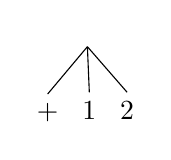
\begin{tikzpicture}
    \Tree [.{ } % Il punto `.` indica un nodo senza testo visibile, ma che può avere figli.
                 % Lo spazio all'interno delle graffe assicura che il nodo esista.
        {+}
        {1}
        {2}
    ];
\end{tikzpicture}
\end{document}
